\documentclass{article}
\usepackage{graphicx}
\usepackage{setspace}
\usepackage{anysize}
\usepackage{fullpage}
\usepackage{natbib}
\usepackage[utf8]{inputenc}
\usepackage{pdfsync}
\usepackage{enumerate}
\usepackage{verbatim}
\usepackage{pdflscape} % makes landscape pages horizontal

% define command to add Celsius degrees
\newcommand{\griddef}[2]{$#1 \times #2^\circ$}

\doublespacing

\title{Range contraction of large pelagic predators in the Pacific \\
  \emph{\large PhD research proposal -- DRAFT}}
%\subtitle{PhD research proposal - Draft}
\author{Laura Tremblay-Boyer}

\begin{document}

\maketitle

\section*{Overview}

\emph{The objective of this PhD thesis is to develop and assess methods to detect
range contraction, explore the impacts of species life-history traits
and dispersal strategies on the relationship between abundance and
range size, and identify key impacts of range contraction on the
 management of fisheries for large, highly mobile species.}

Large pelagic predators such as tuna and billfish play a unique role
in the pelagic communities of the Pacific. They can be both predator
and prey at various stages of their life cycles \citep{Young2010_a,
  Cox2002_a, Hinke2004_a}, occupy a wide range of the water column
\citep{Schaefer2009_a} and store and move important quantities of
carbon and nutrients between coastal and pelagic ecosystems, and along
large distances through their migratory behavior
\citep{Allain2012_a}.

In addition, tuna and billfish fisheries serve as an important source
of proteins to Pacific islands nations, and offer what is often the
only source of foreign revenue to the local economies of these island
states. Many of these species are heavily exploited by modern
fisheries, with more than 60\% of the tuna consumed globally
coming from the Western and Central Pacific \citep{Williams2012_a}.

There has been anecdotal reports from fisheries organizations that
various species of tuna have disappeared from locales where they used
to be abundant (S. Harley, \emph{pers. comm}). Management advice
currently provided to Pacific Islands states does not account for a
potential change in the range of target species and a number of
countries have showed concern in this regard (S. Harley,
\emph{pers. comm}). The optimal strategy for the regional management of
these species would likely be impacted if range contraction was
indeed occuring.

The geographical range of tuna and billfish can be partly explained
through features of the marine environment
\citep[e.g.][]{Reygondeau2012_a}. On small temporal scales they
track specific conditions in the water column like sea surface
temperature, depth of the thermocline, salinity and oxygen
concentration \citep[e.g.][]{Fiedler1987_a, Reese2011_a}. Large-scale
climate cycles that affect these conditions and which are prevalent in
the Pacific (e.g. ENSO, El Nino Southern Oscillation) can thus result
in important changes in the geographic distribution of some of these
species between years \citep{Lehodey1997_a}.

Fishing pressure is another factor that could affect where these
species are found. A recent report indicated that the range of many
tuna and billfish had contracted since the 1970s \citep{Worm2011_a},
although the link to fishing pressure was based on correlative rather
than mechanistic evidence. There are multiple examples from the
conservation literature of range contraction resulting from
over-harvesting \citep[e.g.][]{Laliberte2004_a}. Furthermore, one of the most
important fishery collapse of the 20th century, that of the Atlantic cod,
has been linked to the failure to detect a range contraction in the
species \citep{Rose1999_a}. This failure was in part attributed to the
species' strong schooling instincts, a behavior that is also prevalent
in tuna and billfish.

In this PhD thesis, I intend to assess the potential for range
contraction in large pelagic predators of the Pacific and the
consequences for the management of their fisheries. A key challenge will
be to distinguish whether a change in local abundance is caused by the
environment, an overtly high
fishing pressure resulting in local depletion, or changing
emigration rates enacted through abundance-range size
relationships. To adress this I will merge tools from fisheries
science and marine ecology. The resulting conclusions
will explicitly account for multiple scenarios
of uncertainties through the application of a management strategy
evaluation (MSE). The thesis will be divided as follows:

% Here include one sentence summary for each chapter
\begin{enumerate}[{\tiny $\bullet$}]
\item Chapter 1: Literature review on the topic of the geographic range
across disciplines, with a focus on concepts relevant to highly-mobile
marine species.
\item Chapter 2: Assessement of distribution dynamics in large
  pelagics in the last 60 years using a
low-resolution fisheries catch-and-effort dataset, and impact of data
resolution on inference about abundance trends.
\item Chapter 3: Theoretical population modelling of range-abundance
relationships given life-history features and hypotheses about
dispersal dynamics.
\item Chapter 4: Management strategy evaluation of pelagic predator
fisheries given scenarios about dispersal dynamics, climate change and
management strategies.
\end{enumerate}

I have also included here two potential chapters which
might serve to supplement the thesis if needed.\\

%(Also include diagram of cell immigration/emigration (see draft
%corrected by SJDM))

\newpage
\section*{Chapter 1: Current understanding of species distributions}
\addtocounter{section}{1}

\emph{A literature review will be conducted to (1) identify key
  ecological and evolutionary factors that should be accounted for
  in the measurement and modelling of range contraction, and (2)
  create a framework to synthesize current understanding of the
  geographic range across disciplines.}
\\

% and
%has been a longheld interest of naturalists.
Anthropogenic global change has resulted in drastic changes in the
distribution of many species and, consequently, the last
two decades have seen an explosion of studies aimed at understanding
the drivers of species' distributions. The geographic
range ties in many aspects of a species' biology such that,
unsurprisingly, a variety of approaches have been developed to tackle
the question. Studies, however, often do not account for existing research in
closely-related disciplines. For instance, there is little
cross-pollinization between climate change, conservation and invasive
species research, even though scientists in these fields are all
focusing on some sort of range dynamics, be it shifting, expansion or
contraction.

Moving our focus to marine systems, research on the geographic range
in this realm has been minimal compared to terrestrial
systems. A possible reason could be that species occurrence data are hard to obtain for marine
species due to the nature of their habitat (e.g. museum
records are not available to the extent they are for terrestrial
species) \citep[see][]{Tyberghein2012_a}. Range boundaries for
pelagic species could also be harder to define when viewed from a
 terrestrial standpoint. In fisheries science, changes in species range
 are rarely incorporated explicitly in stock assessments, though this
 is made implicitly through a parameter called catchability
 \footnote{Catchability assumes (usually) that a species' range size stays constant
over time.} \citep{Winters1985_a}. Stock assesment practitioners are
well aware that changes in range can happen, as some
important stock collapses have occurred together with range contraction
\citep[][]{Rose1999_a}.
``Density-dependent habitat selection'' is a popular but largely untested
hypothesis \citep{MacCall1990_a} which posits that intra-specific factors like
competition for resources in varied habitats result in a relationship between
range size and abundance \citep[but see][]{Shepherd2004_a}.

In light of this, the goal of this chapter is to perform a
literature review on the geographic range across the following
disciplines: behaviour, conservation science, ecology, evolution,
fisheries science, genetics and paleobiology. A second aim is to
create a framework to synthesize our understanding of this
literature along three axes: environmental \emph{vs.} biotic
drivers, single \emph{vs.} community effects, marine \emph{vs.}
terrestrial systems.\\
\\
Current status: first draft 95\% completed, need to format for
journal submission (journal to be determined), ideally need a second
author with research experience in topics related to species
distributions.


\clearpage
\section*{Chapter 2: Trends in species range using Pacific-wide CPUE
  data}
\addtocounter{section}{1}
\emph{This chapter aims to develop methods to detect range contraction
  in large pelagics using large-scale coarse resolution spatio-temporal fisheries data,
  as well as highlight features of commonly available datasets that
  could confound measurements of range contraction.}\\

In order to detect range contraction, we need species occurence data that covers the entire
distribution of a species, ideally on a long-term basis. When
these data exist, however, it is often at a coarse scale. Can we make inference
about changes in a species' distribution from such datasets ? What are
the confounding variables that are likely to bias our analysis? In
this chapter I use \griddef{5}{5} aggregated catch-and-effort
data of large pelagics in the Pacific since the
1950s to assess changes in range over time. I assume that catch-per-unit-effort is proportional to
abundance, such that this dataset is effectively a record of large pelagics
occurence in the Pacific over the last 60 years. I start by fitting a statistical model to the existing
data, then use the model to predict the value in cells with years of
missing data. I define a series of arbitrary abundance thresholds above
which the species is considered to be present, and then use these to
detect changes in range area over time. Lastly, I use high-resolution
fishing trip data to verify some of the assumptions made when using
the \griddef{5}{5} data. The trip data only covers a subset of the spatial
and temporal extent of the \griddef{5}{5} data, so this analysis is
applied where the two datasets overlap.

% intro to range contraction
% presence/absence vs changes in occupancy
%For range contraction to have occurred, a species' current geographic
%range must be smaller than its historical range. In other words,
%it must be absent from locales where it used to be present more often
%than in the opposite situation.

Throughout this thesis I will define range contraction as any decline
in the area where a species used to be abundant. This is partly for
practical reasons as we could not tell from the data whether a species
is absent with full certainty. It, however, also has an ecological
justification: it is informative to document instances where the
species went from abundant to rare, since this abundance decline might
(1) be the precursor to extirpation and (2) indicate that ecosystem
dynamics in those locales are likely to be changing. CPUE data
converted to an abundance index could, if used carefully, provide
information about relative abundance over time and be used to assess
changes in occupancy over the range.

% example of work done with presence-absence
%Previous work by \citet{Worm2011_a} has documented a decline in the range of 9
%large pelagics by converting CPUE data from the Pacific to
%presence/absence data. The work in this chapter will go further by
%providing an estimate of change in abundance within the range.
%\noindent \line(1,0){470}

\subsection{Description of the dataset}

Industrial fishing for tuna has taken place in the Pacific since the
1950s, and extensive fisheries catch data exist for this region at
various degrees of spatial and temporal resolution. In its simplest
expression, spatial catch data can be used as a proxy for presence
data. In order to extract additional information, a common approach in
fisheries is to convert catch data to an index of species abundance by dividing
them by a unit of effort (catch-per-unit-effort, CPUE)
(\citealt{Maunder2004_a}, but see \citealt{Harley2001_a}). In this
chapter I use a large dataset of longline CPUE data
to assess range contraction of large pelagics in the
Pacific. The dataset has
been collated by the Secretariat of the Pacific Communities (SPC) and
covers the period 1952-present at a 5 degree
resolution for a range of fishing fleets. Catch data for the following species is
present: yellowfin tuna, big-eye tuna, albacore tuna, skipjack
tuna, southern bluefin tuna, black marlin, blue marlin, striped
marlin, sailfish and swordfish. The time period included in the dataset
covers the history of all major longline fleets. The focus is on
longline data for now as it is the prevalent method of fishing in the
Pacific. Figure \ref{fig1} gives an overview of the dataset for the 6 most
commonly caught species.
% Here SM suggests to show CPUE instead of catch density. DONE.

\begin{landscape}
\begin{figure}
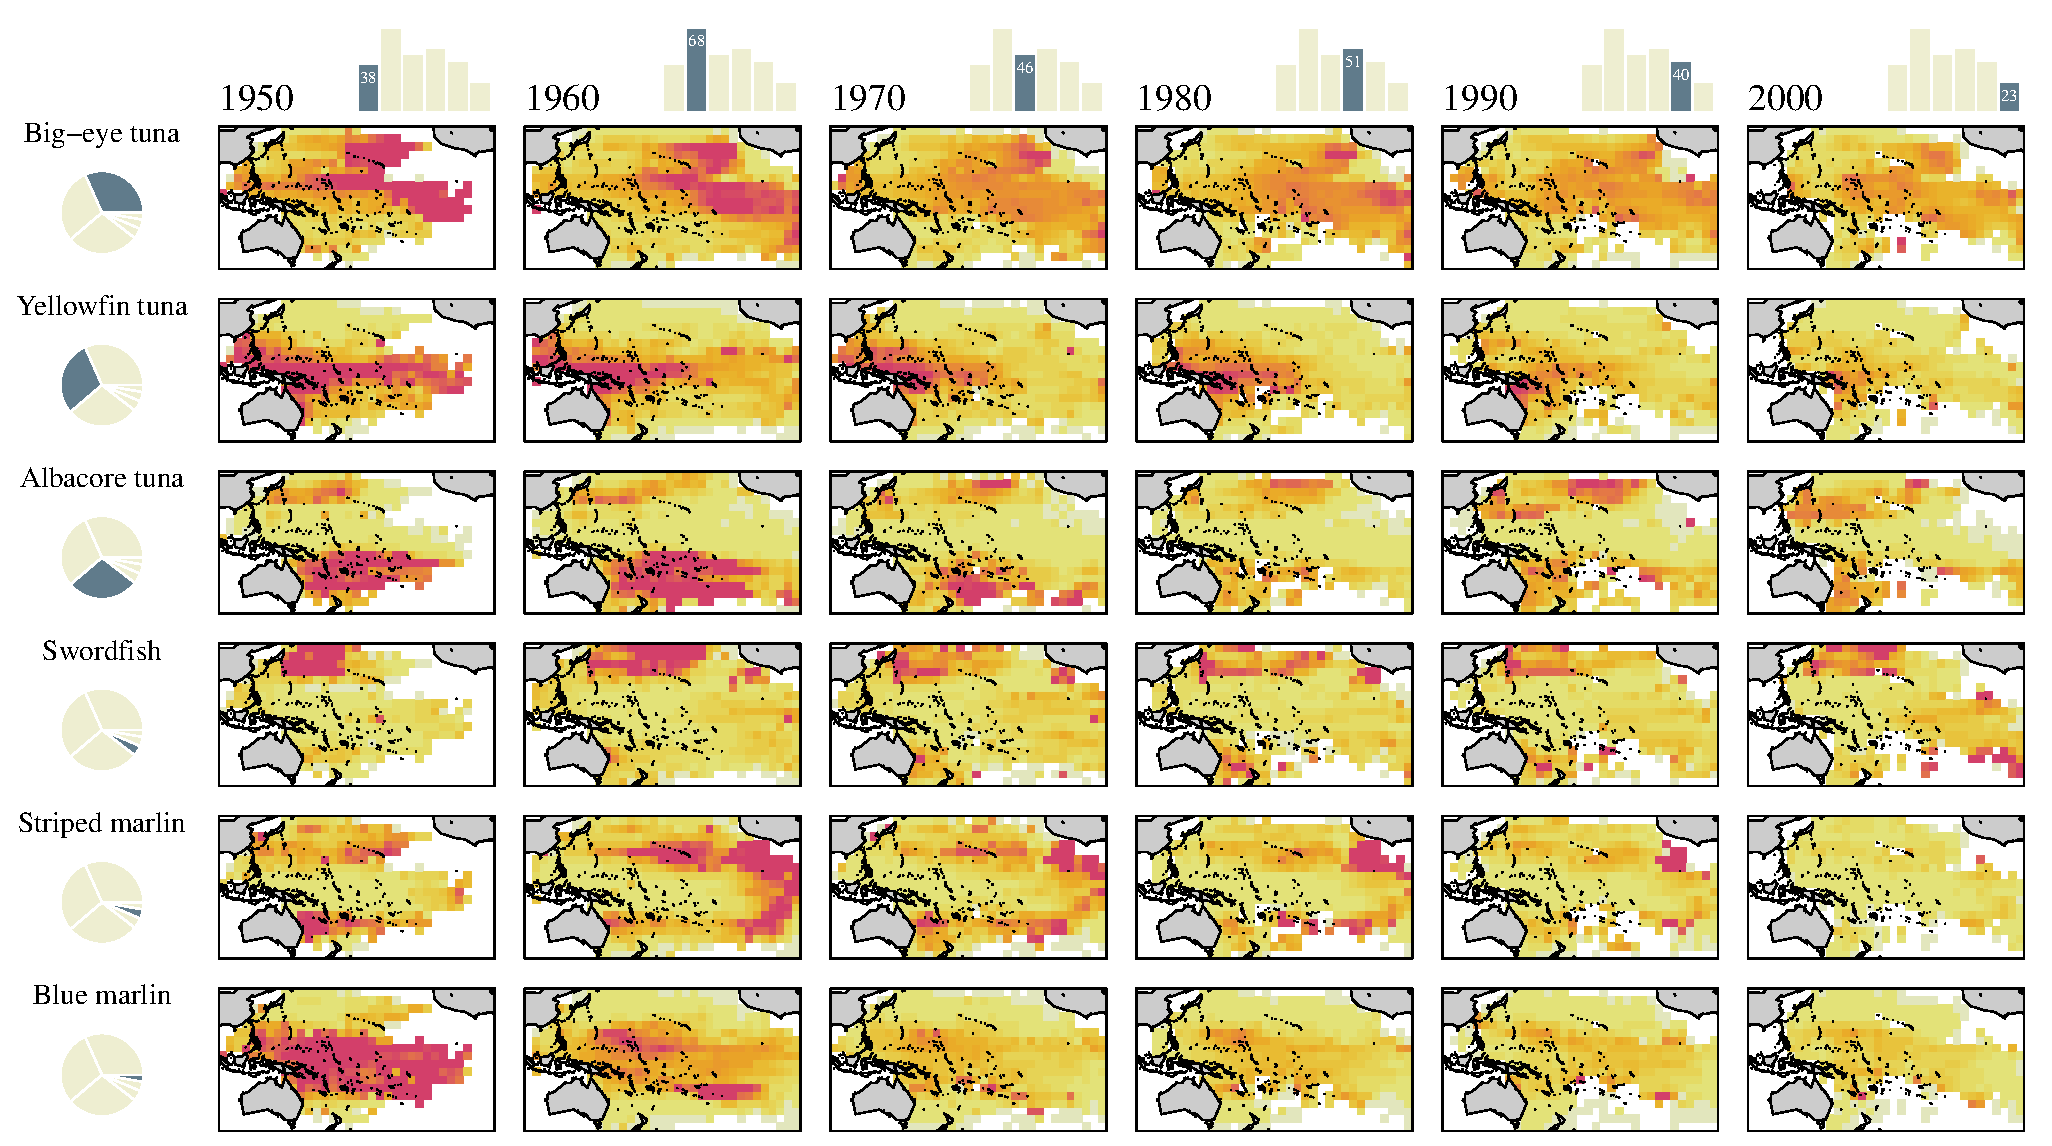
\includegraphics[scale=0.725]{PhD_Proposal_Spring2013_Fig1_nogrid}
\caption{\label{fig1}
Summary of catch-and-effort for the \griddef{5}{5} aggregated data from
  the SPC for the 6 most frequently caught species: Map of relative
  catch-per-unit-effort aggregated over decade and standardized for
  each species; proportion of
  each species in the total catch (left); total catch across species
  by decade  (in million individuals) (top).}
\end{figure}
\end{landscape}

\subsection{Using CPUE as an index of abundance}
% more details about CPUE:
%.

The underlying assumption behind the use of CPUE as
an abundance index is that catch rates are proportional to
abundance. This assumption, however, requires a random distribution of fishing
effort throughout the area where catch data come from. In reality, effort is rarely distributed randomly
over a species' range as fishermen will fish where income is
maximized. In addition, a number of confounding factors prevent raw
CPUE data from being used without further processing (usually in the form of
standardization). For instance, over long time periods, technological
advances in fishing gear increase fishing efficiency, such that CPUE
has a different interpretation today than 3 decades ago. Other issues
associated with the use of CPUE as a measure of abundance are reviewed
in \citet{Harley2001_a}. An active field of research in fisheries
science is to develop methods that yield unbiased indices of
abundance from CPUE data \citep[e.g.][]{Campbell2004_a}, but they
themselves are often heavily criticized
\citep{Carruthers2010_a}. Despite this, fishery-dependent CPUE data do
contain useful information if one is careful and explicit
about the assumptions made in its use. An important challenge in
the current work will thus be to develop analyses that are robust to
the limitations of CPUE data.


\subsection{Predicting CPUE in space and time}
% In this chapter I will use the 5x5 japanese LL dataset to create a
% relative abundance of tuna over the Pacific
% Need to fill the holes in space and time
The \griddef{5}{5} longline dataset available through the SPC arguably
has the largest spatial and temporal coverage for marine
species in the Pacific. Nonetheless, there remain many cells with missing
catch-and-effort data either for a section or the entirety of the
time-series. As pointed out by \citet{Walters2003_a}, the
failure to explicitly consider cells with no fisheries data is a
common error made in CPUE analyses and can lead to wrong inferences
about abundance trends. For instance \citet{Myers2003_a} assumed that
trends in CPUE data for a subset of cells in the Pacific were
representative of overall stock trends and predicted a decline in abundance much
higher than that measured in more involved subsequent analyses
\citep{Sibert2006_a}. Special attention must thus be provided to
filling cells with missing data so that the \griddef{5}{5} dataset can serve
as an unbiased proxy for abundance over the Pacific. Current
approaches to filling in abundance are rule-based, for example
\citet{Carruthers2011_a}, following suggestions by
\citet{Walters2003_a}, used simulated data to test a rule-based
approach to fill-in missing CPUE cell data based on data
existing for that cell in subsequent years. One important advantage with
the rule-based approach is that it is straight-forward to apply and
understand. However, for the approach to be
practical, we are restricted to one dimension: the value of a cell can
only be affected by values of that same cell in future years, even
though data from neighbouring cells in the current year might be
available. In addition, with varying oceanographic conditions, abundance in future
years may or may not be representative of abundance in the current
year. I propose to use a statistical approach to fit spatio-temporal
splines to the existing abundance index and predict the value for
missing cells from the resulting model. The advantage of using splines
is that the relationship of catch over space and time need not be
linear (or a complicated polynomial), and we can retain high degrees
of freedom since longitude and latitude are not treated as fixed
effects. % <--- check this statement!!

 % example of work done with presence-absence
%This should be straightforward to
%measure if one has a time-series of presence/absence data. For
%instance, \citet{Worm2011_a} documented a decline in the range of 9
%large pelagics by converting CPUE data from the Pacific to
%presence/absence data using a simple formula to convert absences from
%the dataset into ``true'' absences. This approach yielded useful
%results, but failed to show whether the occupancy of the locales where
%the species was still present had changed.

% In addition, oceanography data
For the purpose of the current analysis, the main issue to address
with the CPUE dataset is the need to distinguish between an absence of
a species in a cell due to the fishery not having gotten there yet
(i.e. spatial expansion of fishing effort), or
due to the disappearance of the species from a cell where it was
present in the past. The use of oceanography data as a covariate could
address this by providing indication of the likely stock abundance
expected in cells with no effort data given the environmental
suitability. A quick exploration showed that sea temperature and time on
their own explained 45\% of the variance in the \griddef{5}{5} CPUE dataset,
confirming the assertion that oceanographic variables would be good
candidates to inform abundance levels in unobserved cells.

One of the main challenges in fitting a spatio-temporal spline model
to the Pacific-wide CPUE data will be to find an adequate strategy to
account for spatial autocorrelation between the cells and
temporal autocorrelation between the years. So far computing power has
limited the application of conventional methods, since the dataset is
quite large.

%For instance, a current issue in the analysis is that response
%variable is much higher in the tropics than in temperate zone such
%that model error ends up being much higher in high latitudes.

Lastly, to apply this method to all large pelagics, I would have
to account for the different properties that target
and by-catch species have in catch datasets. For instance, effort is
not always linked to abundance for by-catch species such that a CPUE
derived from effort targeted at another species might not yield a
representative index of abundance \citep[see][]{Ortiz2004_a}. A way to address this could be to focus the
analysis on target species only, which would be identified either
through the use of a separate dataset of covariates informative of the
species being targeted \citep[e.g. historical expert opinion,
hooks-per-basket, see][]{Ward2005_a}, or a formal cluster analysis
using disaggregated fleet data that could be used to split the catch
data into subsets where a single species is being targeted.

%Other questions that would be interesting to pursue include the use of
%community data to further inform the observed trends of presence in
%the catch, since some species assemblage tend to be caught together
%more often.

\subsection{Impact of data resolution on measured trends}

%Could also link back to Rabeck et al (2005) and studies on species
%richness.

A second component of this chapter will be to investigate the
sensitivity of results to the scale of data aggregation. \griddef{5}{5}
cells have an area between 230 000 and 310 000 km$^2$ -- the assumption
that CPUE rates averaged at that resolution are representative of
CPUE rates experienced by individual boats is thus an important one. I
have access to two datasets that provide catch-and-effort data at a finer
resolution for the Pacific: (1) operational fisheries data (catch reports by
individual boats); (2) \griddef{1}{1} fisheries data for the Japanese
fleet. Both of these only cover a subset of the spatial and temporal
extent of the \griddef{5}{5} dataset, but can still be used to test
the impact of scale where the datasets overlap.

Overall patterns in catch rates over space and time will be investigated to
see if they match those obtained at a coarse resolution. In addition I
will try to detect patterns of spatial expansion of fishing within
\griddef{5}{5} cells. The latter would inform us about whether
declines might be due to serial depletion of fishing
grounds. This additional work will allow to highlight features of data
resolution that can confound the detection of range contraction, and
also provide support (or not) for patterns detected at the Pacific
basin scale \footnote{if we assume that
differences between fine and coarse dataset for the overlap are
representative of what they would be at the scale of the
Pacific}. Finally, using trip data could allow us to account for targeting
to see whether the cessation of fishing effort in a cell is due to a depletion
of the ressource, or to a change in targeting strategy by the fishermen.
(Include map showing spatial/temporal coverage for both dataset?)\\
\\
Current status: Analysis 95\% done on \griddef{5}{5} for sample
species yellowfin tuna, starting on other species and fine resolution
data, short paper presented to Pacific Islands Forum Fisheries Agency.

%Main issue 1: technology -- however range contraction estimates would be
%conservative
%Main issue 2: targeting (why boats are abandoning cells)

%Lastly, a key issue to address in this chapter will be the interaction
%between climatic drivers and fishing pressure on the realized range of
%tuna and billfish. The use of simulated data and scenarios might be a
%tool to untangle the strength of the influence of one vs. the other.\\

\newpage
\section*{Chapter 3: Population modelling}
\addtocounter{section}{1}
\setcounter{subsection}{0}

\emph{A spatially-explicit population model will be built to
explore the impact of dispersal behaviour and life-history
characteristics on (1) the
relationship between geographic range and population size and (2) the
distribution of biomass in the range as abundance declines.}\\

% chapter overview:
The interpretation of observed spatial trends in the abundance of
large pelagics can be complicated due to (1) the high-mobility of
these species; (2) the prevalence of dynamic oceanographic conditions
in the Pacific; and (3) evolving patterns of fishing
effort. Explicitly including these processes in a
theoretical population model would improve our understanding of the
driving factors behind observed abundance-range size relationships.

In this chapter I will explore the impact of movement, dispersal and
migration behaviour on the range dynamics of large
pelagics. A spatial, environmentally-explicit population dynamics model will
be developed. This model will first be used in a theoretical framework
to understand how assumptions about movement, dispersal and migration
affect observed range dynamics in heterogeneous environments. The
model will then be parameterized using a set
of tropical tunas with different life histories as case-studies
(e.g. skipjack vs. yellowfin vs. bigeye tuna), and accounting for various
spatio-temporal trends in fishing mortality. This will be used to generate
 predictions of biomass distribution in the range as abundance
 declines, which could then be compared to observed
patterns of abundance in space and time obtained in Chapter 2. The
impact of the contraction behaviour on the regional management of
these fisheries will be considered in the next chapter.

%As a last objective, the model could generate some practical predictions
%to explain trends in distribution patterns of some of these exploited
%fish. For instance, what would be the minimum life dispersal
%expectancy for patterns in yellowfin range contraction to be explained
%by DDHS? Givent that most evidence to address this question has to be
%correlative due to the scale of the system, a modelling approach would
%provide an alternative perspective on attemption to resolve this question.

%The goal of that second step will be to identify range
%dynamics that are likely to be expected from these species, and
%highlight parameters to which conclusions are sensitive in order to
%better direct research effort. %example: median dispersal distance

\subsection{Movement, dispersal and migration \emph{vs.} abundance-range size relationships}

The use of habitat by individuals and how that changes with abundance
could have a strong impact on geographic range dynamics. It is obvious that
the range occupied by a critically endangered
species with 10 individuals would be less than that originally
occupied by the population when it was abundant. But what
are the dynamics that drive the geographic range from its initial
extent to the very restricted one expected for a small population?
Dispersal behaviour is a main candidate to explain how some
aspects of this contraction would occur. For instance, if
individuals are sedentary we would expect that geographic contraction
would occur first where mortality is highest. If they are mobile (like
large pelagics), then a process like density-dependent habitat
selection could occur, whereby population contracts towards high
quality habitat as overall abundance is reduced.

The relationship between the abundance of a species and the extent of
its distribution implies that some component of the way invididuals,
groups or populations use their environment is density-dependent. For
instance, consider the case where individuals are randomly distributed
throughout their range (Figure \ref{lili}, left column). If abundance
declines and home range stays constant, then the area of the range
will decline as well, though not as much as if individuals tend to
aggregate (right column). The only way for range size to stay constant
as population declines would be for the home range of individuals to
increase to compensate (left column, bottom).  Density-dependent
dispersal has been documented in a number of species
\citep{Matthysen2005_a} and could be a mechanism through which such
range-abundance dynamics emerge.

In the current chapter I propose to use large pelagics as a model system to
explore how/whether range dynamics can emerge in non-sedentary
populations. Large pelagics are a good case-study to address this
question for the following reasons:
\begin{enumerate}[--]
\item Large pelagics are highly-mobile \emph{and} migratory. These two
behaviours are hard to tell apart when analyzing occurrence
data. Modelling these features will allow us to isolate in a
controlled environment the effect each behaviour has on range dynamics.
\item They represent a range of
life-histories while belonging to similar ecological functional
groups, such that the model could represent a range of species by
tweaking a set of key parameters.
\item A simple spatial model structure would be justifiable since they
  are thought to track smooth gradients in the environment.
\item From a practical perspective, most stocks show an
important decline due to fishing pressure but not so much that their
populations are threatened, i.e. they cover a range of intermediate
values of abundance and, from a management perspective, better
understanding of their range dynamics would be useful \emph{now}.
\end{enumerate}


% description for figure
\begin{figure}[!h]
\label{lili}
\begin{center}
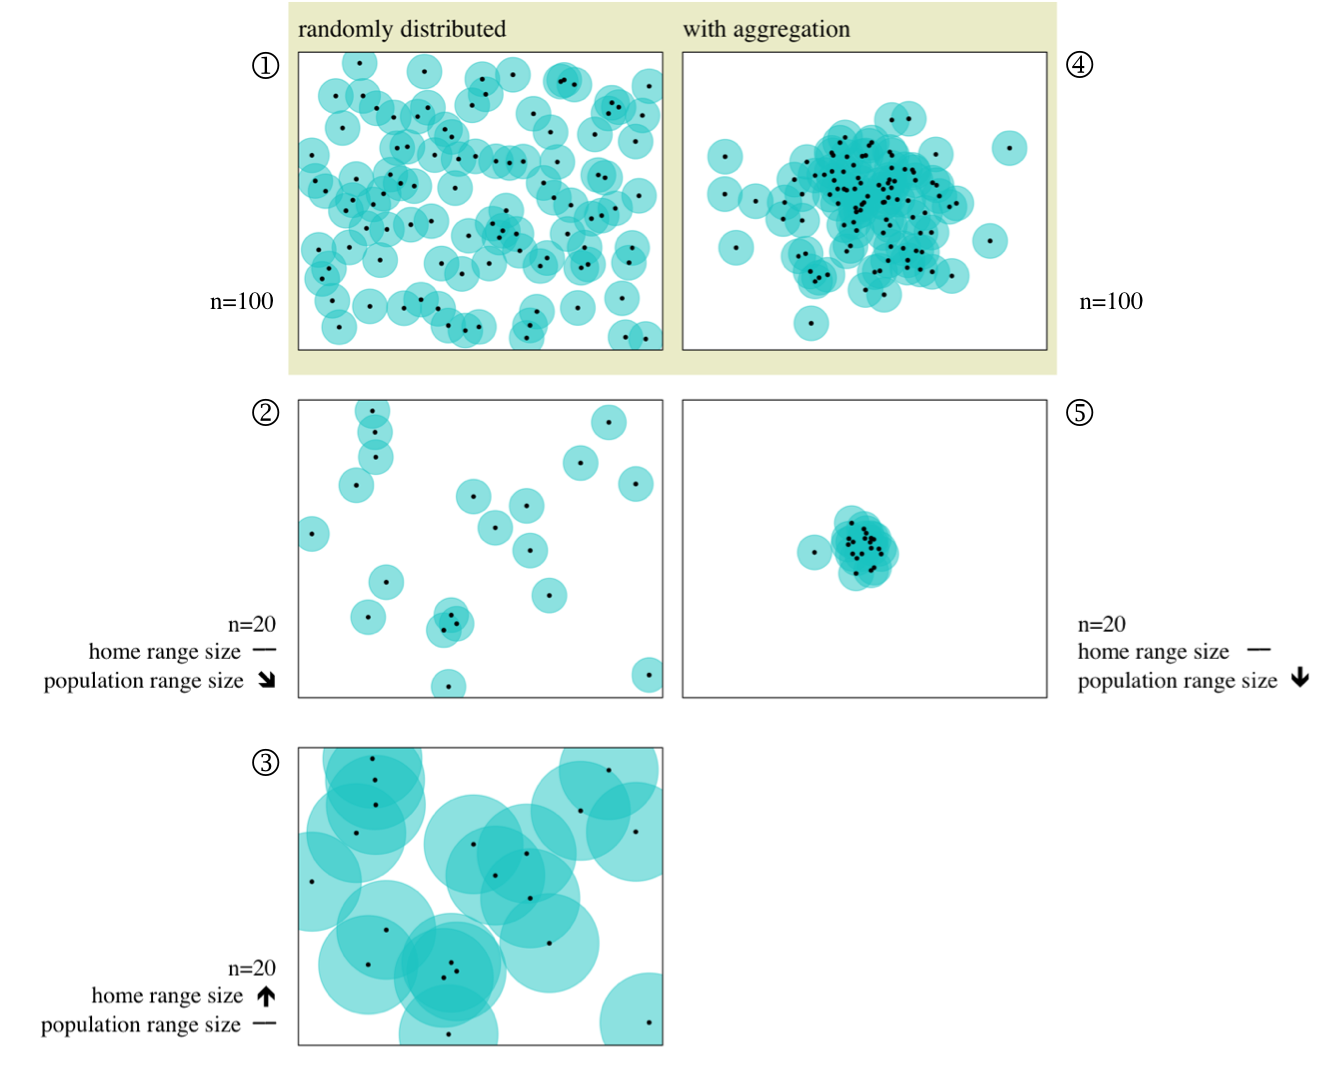
\includegraphics[scale=0.75]{PhD_ResearchProposal_DiagramAreaAbundanceHomeRange2.png}
\caption{Effects on the range of a reduction of abundance of one fifth from
  initial conditions (top, in yellow rectangle), given individuals
  that are randomly dispersed (left column) or aggregated in
  space. The home range of each individuals is represented by the blue
  circles. In cases (2) and (4) home range stays constant as abundance
  diminishes. In the former this results in small reduction in range
  while in the latter the reduction in range is high. In case (3) home
  range size increases such that population range size stays the same
  despite the one fifth decline in abundance.}
\end{center}
\end{figure}

\subsection{The role of fishing in shaping abundance-range size relationships
 of highly-mobile large pelagics}

Fishing pressure is an important driver behind the decline of tropical
tuna biomass and additional mortality incurred through fishing
is not spread evenly throughout the range. Changes in range size with
abundance are thus likely to be affected by both intrinsic
ecological factors and spatial trends in fishing effort. The model
needs to account for this in order to be useful in the analysis of
real-life abundance data from large pelagics in the Pacific. As an
example, Figure
\ref{chap3diag2} shows how abundance patterns for a mobile
fish changes from unfished to fished conditions depending on whether
fish move in a non-random way throughout the range (e.g. migration
towards preferred core habitats) or whether fishing mortality is
higher in locales with higher abundance.

The role of spatial trends in fishing could be explored by applying to
the model simple patterns of fishing effort \citep[as in, for
e.g.][]{Swain1994_a}. Another option would be to extract effort
patterns from the SPC database and use those to drive the model.

\begin{figure}
\label{chap3diag2}
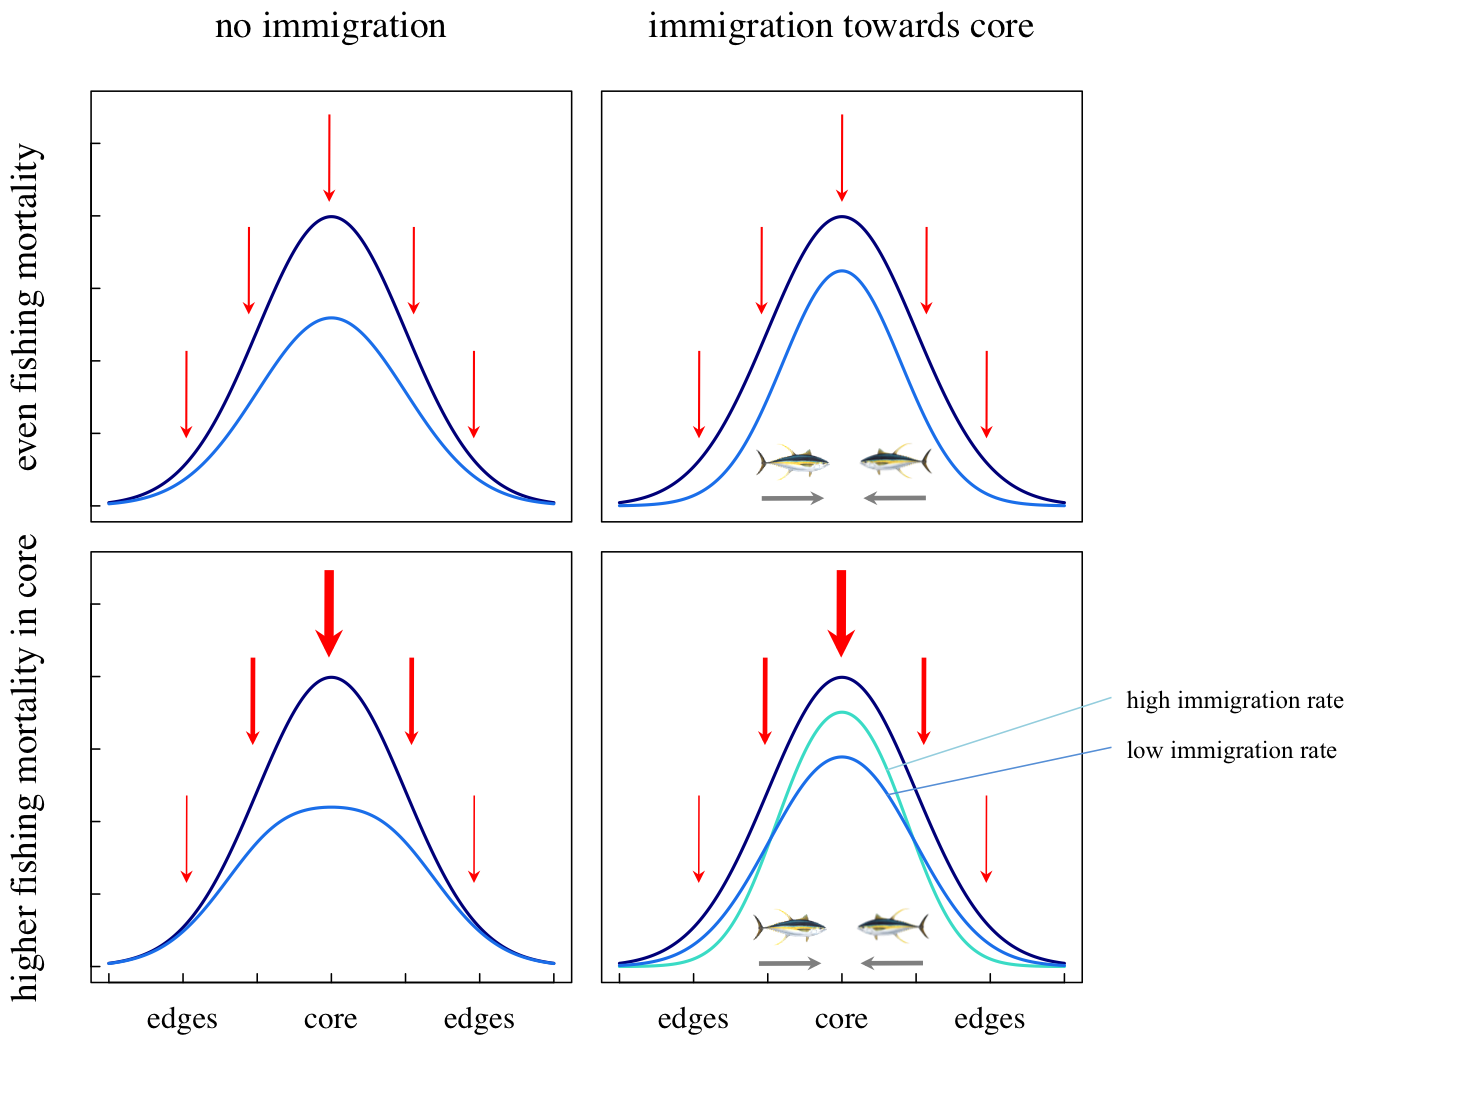
\includegraphics[scale=0.75]{LTB_ResProposal_2013_Chap3_Diagram2.png}
\caption{Schematic representation of the distribution of biomass of
  highly-mobile pelagics in unfished (dark blue line) vs. fished
  (light blue line) conditions as a function of two factors: (1)
  distribution of fishing mortality over
  the range (top, even over the range; bottom, higher at the core) and
  (2) relationship between immigration rates and density in core
  habitats (left, no relationship; right: increase immigration rate
  towards the core when abundance in the core declines). It is assumed
  here that habitat quality is higher at the range core than at the
  range edges. Declines in
  abundance at edges are more
  pronounced when there is increased immigration towards the core,
  though the effect vary as a combination of the difference in
  fishing mortality between the core and the edges and the impact of
  abundance on immigration rates (bottom-right figure).   }
\end{figure}


%Another thing to consider is how the range is measured. For instance
%if the range is the general area where individuals of a species are
%found (e.g. minimum convez polygon containing all points), then
%declines in ranges with abundance will be harder to detect. As an
%illustration, compare the sum of the area of the turquoise circles to
%the area of the polygon that encloses all points in case (2) of figure
%\ref{lili}. The area where the species can actually be found (in
%turquoise) is much smaller than the area covered by the polygon.

%Once the model is developed it can be used to make predictions about
%how biomass declines over the range. Are there life history features
%that make it more likely that the decline is proportional (or not?)

%The Atlantic cod's distribution drastically declined
%under high fishing pressure as aggregation behavior maintained
%individuals closely clustered in space, such that population range
%declined along with abundance. In this case the species is not
%randomly distributed, individuals are clustered together, and home range stays constant
%independently of abundance. This leads to a steep relationship between
%geographic range and abundance. Dispersal would be a key component to
%investigate as any range dynamics hypotheses that relies on ideal free
%distribution should involve home range or dispersal -- since ideal free distribution
%assumes that individuals have perfect knowledge of their
%environment.

\subsection{The iSCAM model}

I propose to use iSCAM as a starting point for the model
\citep{Martell2012_a}. iSCAM stands for ``integrated statistical catch at age
model''. iSCAM is currently under development and is a population
model used in stock assesments, which would make it suitable to model the
CPUE data from large pelagics in the Pacific. I would have to extend
the model to make it spatially explicit on a grid, and include
density-dependent movement/home range/migration relationships. This is
likely to be one of the main challenges in model formulation and will
rely on the definition of a relationship between local abundance and
some form of habitat use by individuals.

\subsection{Comparing model predictions to observed patterns in
  biomass distribution}

Understanding temporal changes in the spatial distribution of biomass
over the range is important for the regional management of
tuna stocks. One of the key modelling results of this chapter will be
the predictions of patterns of biomass distribution in space
and time as a function of life-history and dispersal behaviour. These
predictions can be compared to the modelled abundance obtained in
Chapter 2 in order to understand which mechanisms might be at
play under changes in biomass distribution as abundance declines. In
addition, the model could be used to test different metrics for
measuring changes in the geographic range \citep[for example CPUE
thresholds as done in Chapter 2, and other methods advocated
in][]{Swain1994_a}.

\subsection{Identifying key parameters for research prioritisation}

There is considerable money invested in researching various aspects
of the biology of tuna. An output of this chapter could be to
identify which measurable-in-the-field model parameters have the
largest impact on modelled abundance-range area
relationships. An example of such a parameter is the median lifetime
dispersal distance, which is measured using targeting data
\citep[see for e.g.][]{Sibert2003_a}. This approach could be used to
inform investment into tuna research and be developed into a paper on
conservation/management funds prioritization.

%Lastly, in the case of large pelagics, which are highly mobile,
%migration and dispersal would have to be partitioned.

%More indirectly, individual Eurasian lynx's home range
%increases with lower resource availability \citep{Schmidt2008_aCHECK}.

%Little is know about density-dependent dispersal, especially for
%highly mobile species like large pelagics.

%Complex study system and using a theoretical framework will allow to
%look at various hypotheses, for e.g. impact of migration vs. dispersal.

%This chapter would have two objectives: first I would build a spatial
%population model with an explicit relationship between individuals,
%the space they occupy and population abundance. I would account for a
%variety of life-history characteristics and model what
%abundance-distribution pattern could be expected. The model would be
%as simple as possible to start with, but there are a number of add-ons
%that would be interesting. For instance, an additional avenue to
%explore would be to model dispersal at the adult and juvenile stage.

%For large pelagics: Preferred habitat could be
%identified through tagging data. Some sort of mobility index for each
%species could  be calculated from the tagging data, which would then
%be useful when interpreting results. Another way to identify preferred
%habitat would be to look at the SPC by-catch data and identify groups
%of species that are often found together, such that any knowledge
%about the occurrence of these species could be used in formulating a
%habitat model for other species of interest.

\newpage
\section*{Chapter 4: Range dynamics and the management of tropical tunas}
\addtocounter{section}{1}
\setcounter{subsection}{0}
\emph{This chapter will use management strategy evaluation
  to investigate the impacts of range dynamics on tropical tuna
  fisheries management given scenarios about the drivers of range
  contraction, climate-recruitment relationships and management goals.}

There are uncertainties at all steps of a fisheries' management,
from the data collection to the stock assessment to the policy makers'
decisions and the implementation in real-life. Given that most of these
uncertainties cannot be resolved, our approach to
management should strive to be robust to all possible states of the
system. The goal of a management strategy evaluation (MSE) is to
find a mananagement strategy that fulfills the management goals
independently of the uncertainties we might have about the managed
system's state \citep{Punt2007_a}. Such a procedure is especially
useful in a situation where there are a lot of unknowns in the system
being modelled, where shareholders have conflicting management
objectives and  where components important to management
 interact in non-intuitive ways.

The aim of this chapter is to explore the impacts of range dynamics
on the recommended management strategy for tropical
tuna fisheries in the Pacific. I will draw on the results from
chapters 2 and 3 to identify key uncertainties in the modelling of range
contraction behaviour and population dynamics. The
performance of management strategies will be assessed on a per-region
basis since range contraction will have differential impacts on local fisheries
based on their location in the target species' distribution. The MSE will be conceived in such a way that it
renders the analyses of chapters 2 and 3
more robust. For instance, the effects of structural uncertainty in
the modelled relationship between range size and abundance will be
assessed by including scenarios for various mechanisms of range contraction.

\subsection{What are management strategy evaluations?}

MSEs provide a framework to assess
the performance of a set of management strategies while accounting for
uncertainties at multiple stages of the decision-making process. It
explicitly models all of the steps that go into the management of a
species: modelling, decision-making based on the model's results,
application of decision to real world, etc. (see Figure
\ref{msefig}). Uncertainty can be included
at any stage, in the form of a ``scenario''. For instance the population model could include various
mechanisms for abundance-range size relationships and population
parameters could be related to temperature under a climate change
scenario.

The objective of running a MSE is to identify a management strategy
that performs well across all scenarios. One of the main advantages is that
it requires an explicit formulation of management objectives important
to stakeholders, as these are used to evaluate the success of a
management strategy. Once the MSE has run for all combinations of
scenario and management strategy, the performance of each strategy
across all scenarios and over time can be compared.

\begin{figure}
\begin{center}
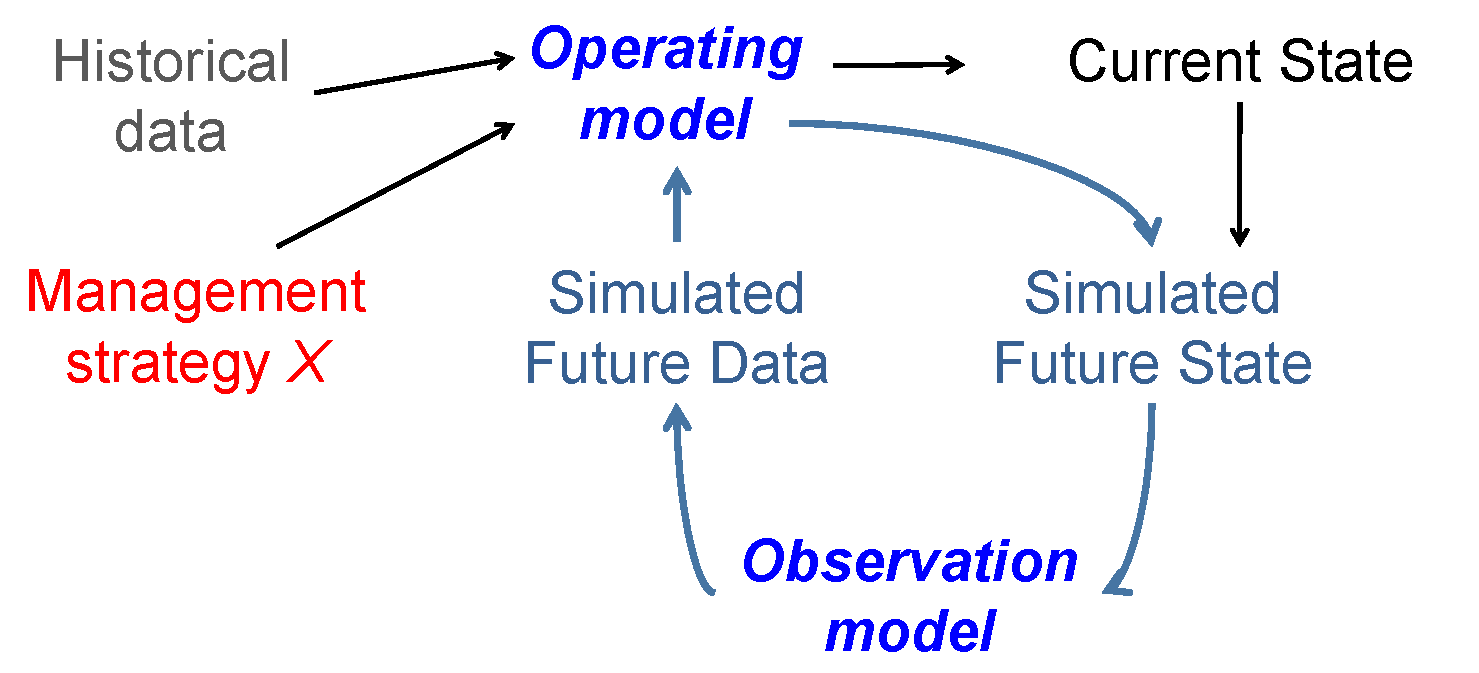
\includegraphics[scale=0.5]{ResearchProposalSpring2013_MSEdiagram}
\label{msefig}
\caption{Flow chart of the modelling component of MSEs. The operating
  model represents population dynamics and is calibrated using
  historical data to product a prediction of what the current state of
  the system is. A management strategy is then applied to the system
  to simulate the state at t + 1. Data is collected from this
  state (e.g. to mimick a fisheries survey) and may include
  observation errors. This collected simulated future data is then
  used in the operating model to predict the state of the system at
  the next time step. This is repeated over a pre-defined time-frame
  for each of the candidate management strategies.}
\end{center}
\end{figure}

\subsection{Applying MSE to range contraction in tropical tunas in the
  Pacific}

The main goal of a MSE here is to evaluate the management impact of uncertainties
about the mechanisms underlying range dynamics as well as assess how
countries might be affected based on the region they are in. The
process will be computationally-intensive so I will focus on a
single species. Yellowfin tuna would be a good candidate here since it
is an important tropical tuna fishery and my preliminary work
indicates that there might be evidence of range contraction.\\
\\
\noindent\textbf{Scenarios:} One of the key challenges in the assessment of
range contraction in large pelagics is to untangle the effects of
local fishing pressure from potential range-abundance relationships
like DDHS. Modelling in chapter 3 should tell us the key parameters
that determine the acting mechanisms and their values
could be used to formulate a set of scenarios. These scenarios are
especially interesting from a regional management perspective as they
would likely result in different recommendations: in the one
instance, abundance at the edges is declining because of high local
fishing pressure, and the other instance abundance at the edges is declining
because fishing pressure in the core is too high.

Other scenarios of interest include the degree of fish mobility, since
there is an ongoing discussion on the consequences of migration of
regional fisheries management, and climate change, as tuna
distribution is sensitive to the environment and this question as been
of interest to member countries.

\noindent\textbf{Operating model:} The population model from chapter 3 would be
used as an operating model.

\noindent\textbf{Observation model:} A simple model could be used whereby
catch-and-effort data is collected and fed back to the stock
assessment. It could be interesthing to explore as a scenario the
effects of input catch data resolution on the recommended
management strategy (e.g. \griddef{5}{5} vs. \griddef{1}{1}
data).

\noindent\textbf{Management objectives:} The management objectives
would be formulated in conjunction with the fisheries staff at the SPC
as well as fisheries representatives from some of the countries, but
would at least include sustainable exploitation of the stocks and some
harvesting objective tied to catch or revenue. There could be some
objectives tied to specific area, e.g. keep catch rates at a certain level
 in edge areas of the range.

\noindent\textbf{Management strategies:} Management options would also be
formulated in consultation with the SPC and could include both
Pacific-wide and region-specific harvest rules. It would also be
interesting to include at least one typical ``conservation''
strategy, e.g. stopping fishing in certain areas/times, given that
there has been a lot of high-profile debate about the potential
benefits of marine reserves for the management of highly migratory tuna
in the Atlantic.

%More details, e.g. MCMC?
%MSE good way to explore structural uncertainty.

\newpage
\section*{Optional chapter 1: Interactions between industrial and artisanal
  fisheries}

One of the main socio-economic consequences of ecology-driven range
contraction is that local catch rates could be impacted by fishing
fleets far away. This is especially relevant to island nations that
rely on pelagic fisheries as an important source of their daily
protein intake. Often these countries have important artisanal fleets
that provide seafood to the local market. The objective of this
chapter would be to develop metrics to assess the interaction between
industrial and artisanal fisheries in countries likely to be affected
by range contraction.

I would use French Polynesia as a case study as they have been
collecting fisheries data on their artisanal fleet since 1997 and have
agreed to provide access to their dataset. French Polynesia consists
of a set of archipelagos located in the south-east of the Pacific and distant
from the core of most tropical tuna species.

Interactions between artisanal and industrial fleets can be direct
and indirect. Direct interaction can occur when industrial fleets
deplete ressources near islands, or prevent artisanal fishermen from
fishing in certain locales. Indirect interaction can occur when
industrial fleets affect the stock at the scale of the Pacific and
impact catch rates of highly-mobile species targeted by artisanal
fisheries. Note that the former is not necessarily linked to range
contraction, but is an important way by which island nations are
impacted by industrial fishing.

Methods to assess interactions would vary between direct and indirect
effects. In the case of direct interactions, an option could be to
develop an index of species overlap (since, presumably, the interaction would be
highest when targeted species are the same). This could be combined
with a proxy for spatial interaction based on the location of industrial fishing
effort as a function of its distance to the coast and weighted by the
number of people living on the island of interest.

To assess indirect interactions, local catch rates could be modelled together
with Pacific-wide stock status indices in order to identify which
proportion of the variation in local catch rates can be explained by
signals from overall stock levels.

Current chapter status: This is a report that I am preparing for the government of
French Polynesia (FP) (the project is coordinated by the SPC), to be
submitted in the Fall of 2013. I have done a first exploratory trip to
FP in March 2013 in which I worked with local fisheries scientists and
did an extensive exploration of the artisanal catch dataset. I came
back a month later to present a preliminary research strategy for the
project to the fisheries department and we agreed on the future
analyses suggested above (though there is some flexibility). The
planned report adresses a wide array of questions but will
likely not go in too much depth due to the short time-frame. The
analyses would have the potential to be further developed into a
full-fledged chapter, keeping in mind that the topic has to be framed
in the context of the overall thesis. I have the permission from the
fisheries department in French Polynesia to use this work as a
chapter.


\newpage
\section*{Optional chapter 2: Using occupancy modelling to detect changes in
  species distribution}

Fisheries catch records arguably constitute the most extensive set of
occurrence data for marine species in space and time. A common
approach in fisheries science is to use the ratio of catch over
fishing effort (catch-per-unit-effort, CPUE) as an index of abundance.
However, fishing trips can also be seen as monitoring surveys which
record species' presence in a given locale, that is, fishing
trips collect presence data.

%If a given species was
%caught during the fishing trip, then we know for sure that it was
%present (if we ignore identification errors). A species' absence from
%a trip is a pseudo-absence because it either indicates true absence of
%the species, or the failure to observe (capture) it when it is in fact
%present.

Range contraction can be shown by measuring faster decline rates in
certain parts of the range than others. Equivalently, a decline in
time of the probability for a species to be present in a
previously-occupied parts of its range would also indicate range
contraction. Methods to detect such a change have been developed
extensively in the climate change and exotic species literature, but
few have been applied to marine problematics \citep{Robinson2011_a}.

In chapter 2 I use CPUE data as a proxy for abundance and
quantify range contraction in large pelagics at the scale of the Pacific
since the 1950s. There are, however, many confounding effects that
hinder the use of CPUE data to infer trends in abundance over time. In
addition, one of the main issues to resolve is whether contraction is
caused by local depletion or ecological population-wide effects like
DDHS. The low spatial resolution of the \griddef{5}{5} dataset makes
it hard to investigate these hypotheses more closely.

Operational data (fishing records at the scale of individual trips)
are available for some regions of the Pacific, in some instances since
the 1970s. These trips could be considered like individual surveys,
and their catch effectively constitute presence-absence data that can
be examined for trends over time. Occupancy modelling is a statistical
framework recently developed in conservation science to examine
presence data and calculate the probability of an absence being real
given repeated surveys \citep{Mackenzie2006_a}. One of the
advantages of using a presence-absence approach is that trends would
be less affected by factors that usually confound CPUE analyses, as we
would not be looking at how much of a species is in a given locale,
but whether it is present there or not. This method would have to be
adjusted to work in a fisheries context, but could provide a novel way
to assess range dynamics in fished species and serve to investigate
candidate mechanisms for range contraction.  In addition,
used together with the results of Chapter 2, it would yield more
robust estimates of range dynamics in large pelagics in the Pacific.

%In addition, while the temporal and spatial extent is more limited, the
%higher resolution could allow to look more specifically for some of
%the predictions made by each hypothesis:

%Under DDHS: faster decline in less optimal habitat once fishing effort
%is standardized out -- the operational data covers a range of habitat
%so should uncover that.

%Under local depletion: declines in probability of occurrence would be
%linked to local fishing effort.

%Challenges: - how to treat fisheries trips as repeated surveys
%(cluster analysis?)
%- accounting for environmental information in occupancy modelling
%- also: fisheries drivers has been applied successfully to blue marlin
%\citep{Su2012_a} so it might be possible to extend a comparable
%methodology to other tuna and billfish.

%Current status: still exploring ideas for this chapter, exploration
%of operational trip data started in June 2013.

\newpage

\singlespacing
\bibliographystyle{apalike}
\bibliography{TremblayBoyer_ResearchProposal_O&I_Biblio}


\end{document}